\begin{frame}
    \frametitle{Terminology}
    \framesubtitle{Generative Adversarial Networks(GAN)}
    \begin{figure}
        \centering
        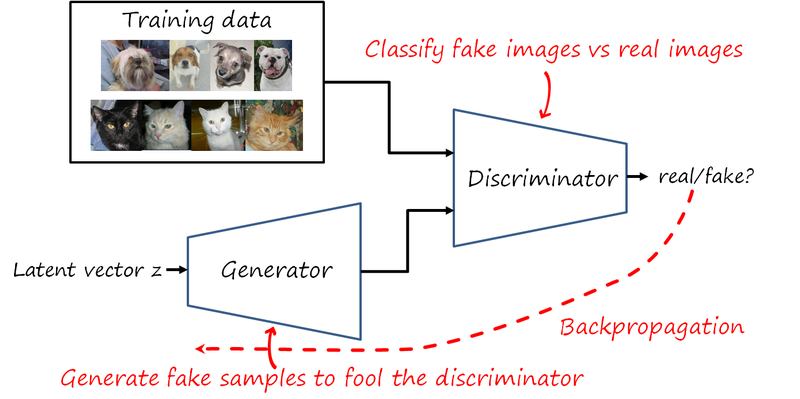
\includegraphics[width=0.65\linewidth]{images/blog_gan.png}
        \caption{GAN training process}
    \end{figure}
    \tiny{\footnotemark \url{http://www.lherranz.org/2018/08/07/imagetranslation/}}
\end{frame}
\note{
    \begin{itemize}
        \item Generative Adversarial Networks: Zwei Netzwerke, Generator und Diskriminator, die gegeneinander trainiert werden        
            \begin{itemize}
                \scriptsize\item Generator: versucht die verteilung der Trainingsdaten zu lernen ohne diese zu kennen
                \scriptsize\item Diskriminator: Unterscheidet zwischen echten und generierten Bildern        
            \end{itemize}            
        \item Loss Function: Min-Max Game zwischen Generator und Diskriminator 
    \end{itemize}
}

\begin{frame}
    \frametitle{Terminology}
    \framesubtitle{Generative Adversarial Networks(GAN) - Loss Function}
    \begin{block}{GAN Loss Function}
        
        \begin{equation}
            \min_G \max_D \mathcal{L}(D,G) = \mathbb{E}_{x \sim p_{\text{data}}(x)}[\log D(x)] + \mathbb{E}_{z \sim p_z(z)}[\log(1 - D(G(z)))]
        \end{equation}
    
    \end{block}
    \tiny{\footnotemark \url{http://www.lherranz.org/2018/08/07/imagetranslation/}}
\end{frame}
\note{       
    
    \begin{itemize}
        \item x: echtes bild
        \item z: Zufälliger Input für den Generator
        \item $p_{\text{data}}(x)$: Wahrscheinlichkeitsverteilung der echten Daten
        \item $p_z(z)$: Wahrscheinlichkeitsverteilung des zufälligen Inputs
        \item $D(x)$: Wahrscheinlichkeit, dass x ein echtes Bild ist
        \item $G(z)$: Generiertes Bild                        
    \end{itemize}
    Diskriminator wird trainiert um die Wahrscheinlichket, dass korrekte Label zu erkennen zu maximieren.\\
    
    Probleme: Früh im Training ist der Generator noch sehr schlecht, deswegen wird der $log(1 - D(G(z)))$ Term sehr groß und der Gradient verschwindet.\\
    In Praxis wird $logD(G(z))$ verwendet, um dieses Problem zu umgehen.\\ 
    
    Weiterentwicklungen: DCGANs, Wasserstein Distance als Loss Function oder PG-GANs nur Name dropping

}
    
% ---------- CycleGAN ----------
\begin{frame}
    \frametitle{Terminology}
    \framesubtitle{CycleGAN}
    \begin{figure}
        \centering
        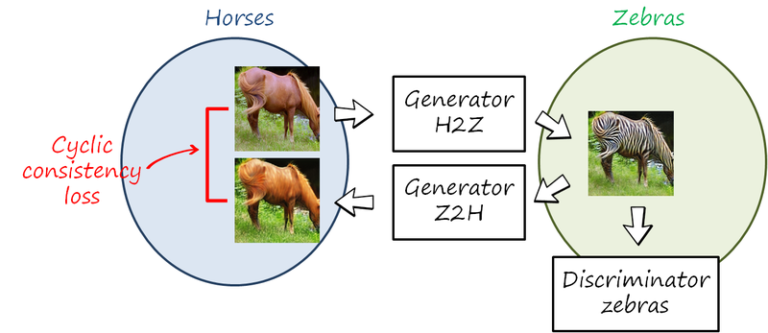
\includegraphics[width=0.78\linewidth]{images/blog_cyclegan_h2z2h-768x333.png}
        \caption{CycleGAN Architecture}
    \end{figure}
    \tiny{\footnotemark \url{http://www.lherranz.org/2018/08/07/imagetranslation/}}
\end{frame}
    
    
        
% ---------- UNet and Skip Connections ----------
\begin{frame}
    \frametitle{Terminology}
    \framesubtitle{UNet and Skip Connections}
    \begin{figure}
        \centering
        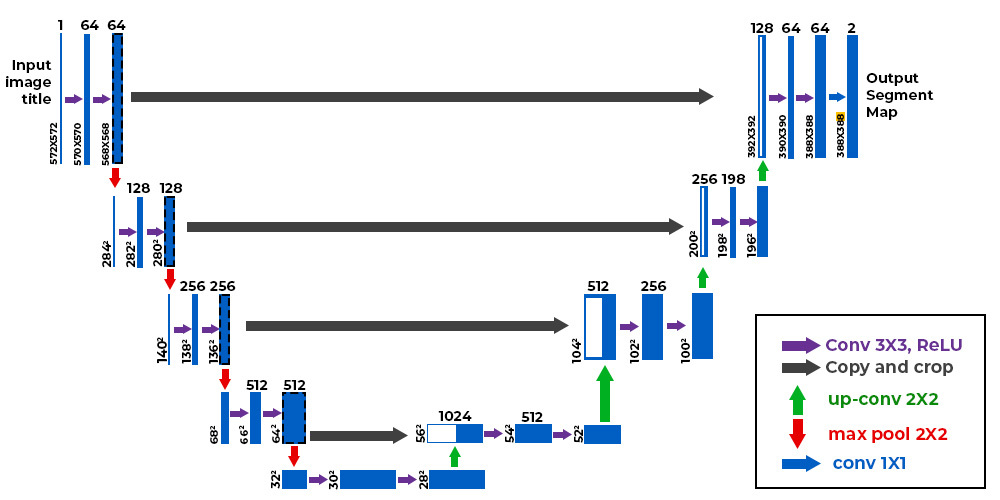
\includegraphics[width=0.6\linewidth]{images/Group14.jpg}
        \caption{Architecture}
    \end{figure}
\end{frame}
\note{
    \begin{itemize}
        \item UNet: Convolutional Neural Network, das für Bildsegmentierung verwendet wird
        \begin{itemize}
            \item Encoder Pfad: Mehrere Blöcke von convolutional layers mit ReLU activation und max pooling. Reduziert die Dimensionalität des Inputs
            \item Decoder Pfad: Mehrere Blöcke von convolutional layers mit RelU activation und upconvolution. Erhöht die Dimensionalität des Inputs. Außerdem Concatenation mit entsprechenden Encoder Pfad
            \item Skip Connections: Verbindung zwischen Encoder und Decoder Pfad. Hilft details zu erhalten, die im Encoder verloren gehen würden
        \end{itemize}
    \end{itemize}
}
    
% ---------- LoRA Weights ----------
\begin{frame}
    \frametitle{Terminology}
    \framesubtitle{LoRA Weights}
    \begin{figure}
        \centering
        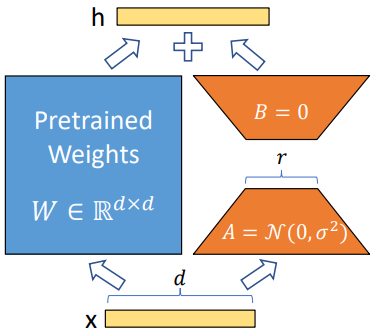
\includegraphics[width=0.4\linewidth]{images/Bildschirmfoto vom 2024-04-15 10-21-59.png}
        \caption{\textbf{Lo}w \textbf{R}ank \textbf{A}daption}
    \end{figure}
\end{frame}

% ---------- Paired vs unpaired data ----------
\begin{frame}
\frametitle{Terminology}
\framesubtitle{Paired vs unpaired data}
\begin{columns}
    \column{0.5\textwidth}
    \centering    
    \begin{figure}
        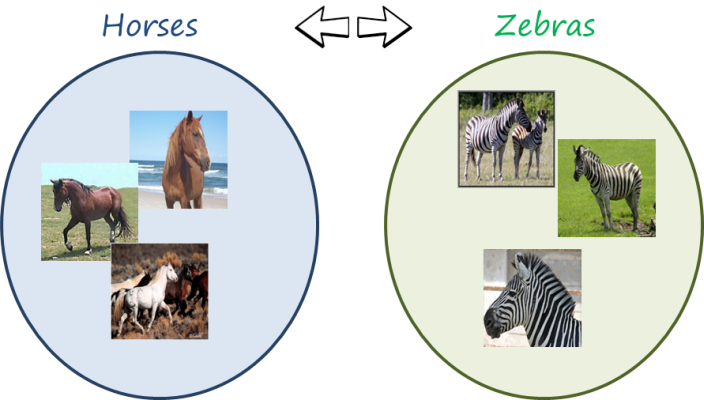
\includegraphics[width=0.75\textwidth]{images/blog_unpairedimagetranslation2.png}
        \caption{Unpaired Data}
    \end{figure}

    \column{0.5\textwidth}    
    \centering    
    \begin{figure}        
        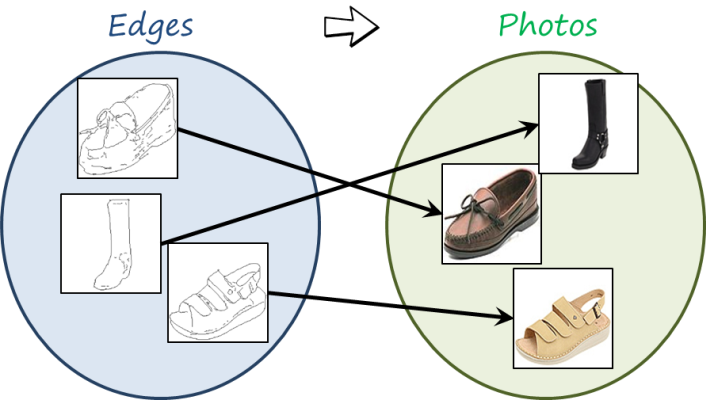
\includegraphics[width=0.75\textwidth]{images/blog_pairedimagetranslation.png}
        \caption{Paired Data}
    \end{figure}
    \end{columns}
\end{frame}
\note{
    \begin{itemize}
        \item Paired data: Jedes Bild in Domain X hat ein korrespondierendes Bild in Domain Y
        \item Unpaired data: Es gibt keine direkte Zuordnung zwischen den Bildern in Domain X und Domain Y
    \end{itemize}

}
